\chapter{Atmel AVR}\label{atmel-avr}

\section{Introduction}\label{avr-introduction}

The Atmel AVR is the micro controller at the heart of your \index{Arduino}Arduino and comes in many different varieties. We are concentrating, in the main, on the Atmel ATmega328P which is the micro controller on the Duemilanove, the UNO and the Nano - although the Nano uses a surface mount version of the 328.

Some clones may also use the surface mounted version of the 328 - it depends. The \index{Arduino}Arduino hardware is open source, so anyone is able to build their own clones, using whatever equivalent micro controllers they can source.

\section{Data Sheets}\label{data-sheets}\index{Data Sheets}

You should, if you have not already done so, download the full data sheet for the ATmega320P from \href{http://www.atmel.com/Images/Atmel-42735-8-bit-AVR-Microcontroller-ATmega328-328P_Datasheet.pdf}{Atmel's web site} - don't worry about the fact that the document is over 440 pages long, we \emph{won't} be reading it from start to finish!

Normally, it's good to get an overview of the micro controller, especially when it's new to us, by reading  through the first few chapters which describe the micro controller and it's registers and features etc.

We will not labour the point here. The data sheet contains all you need to know, and much, much more. 

\section{ATmega328P Pinout}\label{atmega328p-pinout}
Figure~\ref{fig-atmega328p-pinout}, taken from the current data sheet,  shows details of the ATmega328P's various pins. You will notice that there is no mention of the \index{Arduino}Arduino's pins D0 through D13, nor of pins A0 through A5, so perhaps Figure~\ref{fig-arduino-uno-pinout} will help, as the \index{Arduino}Arduino pin usage is shown in red text down each side of the diagram. (Image courtesy of \href{https://www.arduino.cc/en/Hacking/PinMapping168}{www.arduino.cc})

\begin{note}
	You will note that Figure~\ref{fig-arduino-uno-pinout} mentions the \index{ATmega168}ATMega168 rather than the \index{ATmega328P}ATmega328P - don't worry, they are pin compatible. The pins on one micro controller are the same, and have the same functions, as those on the other. They just have different amounts of memory - flash, EEPROM and SRAM.
\end{note}	

\begin{figure}[p]
	\centering
	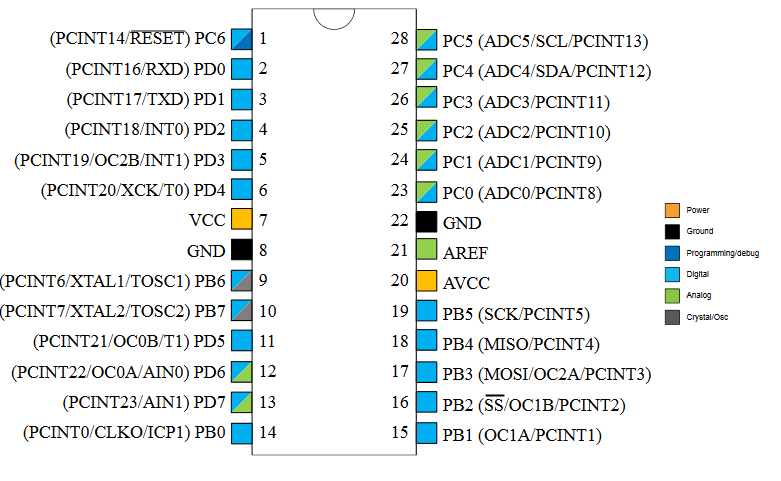
\includegraphics[width=0.9\textwidth]{Content/images/ATmega328P-pins}
	\caption{Pinout Diagram of the ATmega328P Micro Controller}
	\label{fig-atmega328p-pinout}
\end{figure}

\begin{figure}[p]
	\centering
	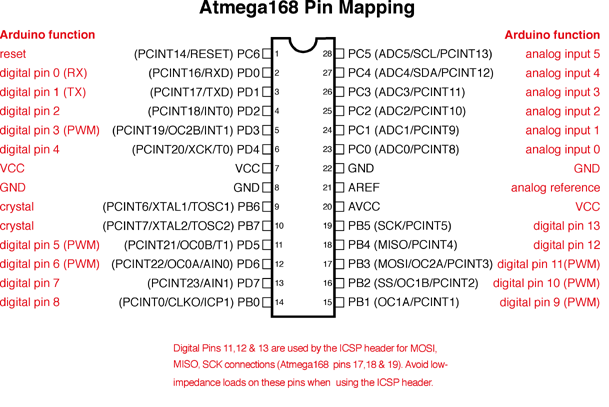
\includegraphics[width=0.9\textwidth]{Content/images/ArduinoUno-pins}
	\caption{Pinout Diagram of the ATmega328P showing Arduino Pin Use}
	\label{fig-arduino-uno-pinout}
\end{figure}

You may be wondering how, if the AVR pinout diagram shown in Figure~\ref{fig-atmega328p-pinout} doesn't have the Arduino's pin definitions, how the Arduino software is able to use the correct pins? This will be explained in section~\refname{avr-pinmodes} on page~\pageref{avr-pinmodes}.

\section{AVR Pinmodes}\label{avr-pinmodes}

You are most probably familiar with the \index{Arduino}Arduino's \inline{pinMode()} function, which allows you to define whether a pin is to be configured as input, output or input with pullup. You will not be surprised to find out that the AVR has a similar feature, but this one can do many pins at once.

However, as mentioned above, you may be wondering how the  \index{Arduino}Arduino software gets from the \index{Arduino}Arduino pin numbering format to those used on the actual AVR hardware? The process  as followed by \inline{pinMode()}, is as follows:

\begin{itemize}
	\item Convert the pin number to a \emph{bit mask} by calling \inline{digitalPinToBitMask()}.
	\item Convert the pin number to a port as well, by calling \inline{digitalPinToPort()}. If the port is invalid, do nothing and exit.
	\item Convert the (valid) port to a mode register by calling \inline{portModeRegister()}.
	\item Convert the (valid) port to a port output register by calling \inline{portOutputRegister()}.
	\item Preserve the current status register for the micro controller. Amongst other details, this will record the current state of the interrupts - whether or not they are currently enabled\footnote{See the data sheet for details of what the Status Register contains.}.
	\item Turn off any interrupts, even if already off. See \href{http://code.google.com/p/arduino/issues/detail?id=146}{This issue} for details of why this has to be done.
	\item Set the pin according to the desired mode - INPUT, INPUT\_PULLUP or OUTPUT.
	\item Restore the status register. This will also re-enable the interrupts, if they were enabled earlier.
\end{itemize}

That's an awful lot of work just to set a pin as OUTPUT, for example.

The functions \inline{digitalPinToBitMask()}, \inline{digitalPinToPort()}, \inline{portModeRegister()} and \inline{portOutputRegister()} are defined in the file:

\fbox{\inline{hardware/avr/cores/arduino/Arduino.h}}

which is located underneath wherever your \index{Arduino}Arduino software is installed. If you ()only) have \index{PlatformIO}PlatformIO installed, then the definitions are in:

\fbox{\inline{/home/norman/.platformio/packages/framework-arduinoavr/cores/arduino/Arduino.h}}

So, how does all of the above get us from the pin number 13, for pin D13, for example, to PB5? Well, the next section explains Ports and Pins, but briefly, calling \inline{pinMode(13, OUTPUT)} does all of the following:

\begin{itemize}
	\item \inline{digitalPinToBitMask(13)} returns a binary value of 0010 000, which is an 8 bit value, with bit 5 set to 1 and all other bits set to 0.
	\item \inline{digitalPinToPort(13)} returns the value 2, which is defined as a constant named ``PB''.
	\item \inline{portModeRegister(PB)} returns a pointer, this is C code remember, to the ``DDRB'' register. More on this in the following section.
	\item \inline{portOutputRegister(PB)} returns a pointer to ``PORTB''. More below on this too.
	\item Saves the status register.
	\item Turns off interrupts.
	\item Binary ORs the required bit of the ``DDRB'' register, bit 5 as above, with a 1, to set the pin to an output.
	\item Restores the status register (and interrupt state).
\end{itemize}

As I said, that's a lot of work, and a lot of code. In addition, there are a number of data tables written to the flash memory, where your program lives, to enable the above function calls to be facilitated. These tables take up $(3 * 10) + (3 * 20)$ or 90 bytes of potentially valuable program space.

That's for the \index{Arduino}Arduino. For plain AVR C code, we set D13 (aka PortB, Pin 5) as follows:

\begin{lstlisting}[numbers={none}]
	DDRB |= (1 << 5);
\end{lstlisting}

Which is a lot less work, a lot fewer bytes overall and no tables are required. However, \emph{we}, the programmer, do have to remember the pin numbers etc.

The following section goes into greater detail about Pins and Ports.

\section{AVR Ports and Pins}\label{avr-ports-and-pins}

\section{}\label{}
